Broken Link Checker\footnote{\url{https://www.brokenlinkcheck.com} (Diakses pada 30 Agustus 2025)} adalah sebuah situs web yang digunakan untuk mendeteksi tautan rusak, baik tautan internal maupun eksternal pada sebuah situs web.


\subsubsection*{Tampilan dan Interaksi}

Gambar~\ref{fig:analisis-brokenlinkchecker} menunjukkan antarmuka Broken Link Checker saat proses pemeriksaan berlangsung. Alur penggunaan secara umum dimulai dengan memasukkan alamat situs pada kolom input, mengisi kode keamanan, memilih mode pemeriksaan, lalu menekan tombol \textit{Find broken links now!} untuk memulai proses. Selama pemeriksaan berjalan, hasil ditampilkan langsung dalam bentuk tabel, dan pengguna dapat menghentikan proses dengan menekan tombol \textit{Stop}.

\begin{figure}[H]
    \centering
    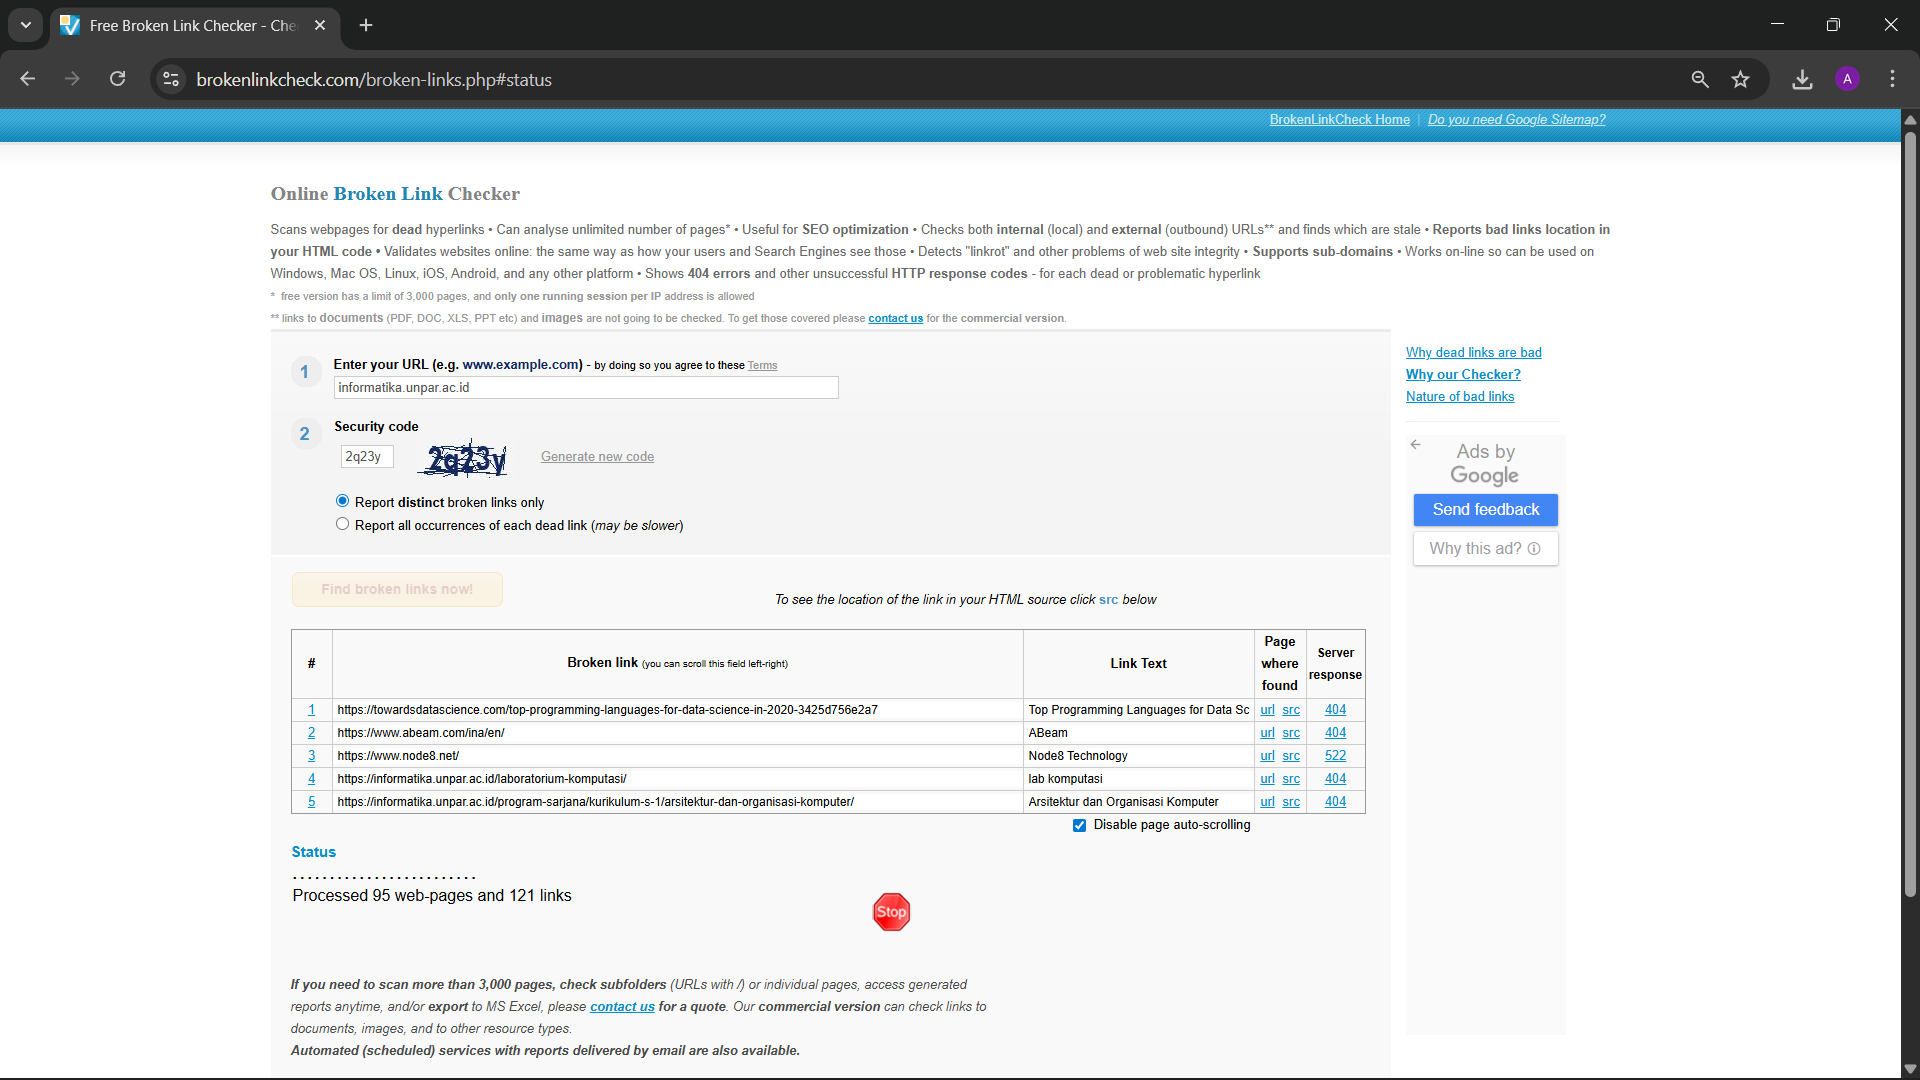
\includegraphics[width=0.95\textwidth]{Gambar/030203-broken-link-checker.png}
    \caption{Antarmuka Broken Link Checker}
    \label{fig:analisis-brokenlinkchecker}
\end{figure}

Berikut adalah komponen utama antarmuka pengguna Broken Link Checker pada layanan pemeriksaan tautan rusak:

\begin{enumerate}
    \item \textbf{Input URL}\\
    Komponen ini digunakan untuk memasukkan alamat situs web yang akan diperiksa. Pengguna dapat menuliskan alamat dalam bentuk domain saja, tanpa harus menyertakan skema \texttt{http://} atau \texttt{https://}. Sistem akan tetap menerima input tersebut dan mengolahnya sebagai URL awal pemeriksaan. Kemudahan ini mempersingkat proses input, meskipun dapat menimbulkan potensi ambiguitas pada situs web yang hanya mendukung skema tertentu, misalnya hanya \texttt{https://}.

    \item \textbf{Security code}\\
    Sebelum memulai proses pemeriksaan, pengguna diwajibkan mengisi \textit{security code} berupa captcha. Keharusan ini berfungsi sebagai mekanisme pencegahan terhadap penggunaan otomatis (bot) yang dapat membebani server layanan. Kode keamanan ini bersifat dinamis dan dapat diganti dengan menekan tombol \textit{Generate new code} yang tersedia pada antarmuka.

    \item \textbf{Mode pemeriksaan}\\
    Tersedia dua pilihan mode pemeriksaan yang dapat dipilih melalui tombol radio, yaitu \textit{Report distinct broken links only}, dan \textit{Report all occurrences of each dead link}. Mode \textit{Report distinct broken links only} menampilkan setiap tautan rusak hanya sekali, tanpa memperhatikan berapa banyak halaman yang memuat tautan tersebut. Pendekatan ini membuat proses lebih cepat, tetapi informasi lokasi kemunculan tautan hanya terbatas pada satu halaman. Sebaliknya, mode \textit{Report all occurrences of each dead link (may be slower)} menampilkan seluruh kemunculan tautan rusak beserta halaman sumbernya. Dengan demikian, jika sebuah tautan rusak terdapat pada beberapa halaman, maka akan muncul beberapa entri dengan sumber berbeda pada tabel hasil. Mode ini memberikan informasi yang lebih lengkap, namun membutuhkan waktu pemrosesan yang lebih lama.

    \item \textbf{Tombol kontrol}\\
    Proses pemeriksaan dimulai dengan menekan tombol \textit{Find broken links now!}. Setelah pemeriksaan berjalan, tombol \textit{Stop} berwarna merah akan muncul di bawah tabel hasil. Tombol ini memungkinkan pengguna menghentikan proses pemeriksaan kapan saja sesuai kebutuhan. Selain itu, disediakan pula opsi \textit{Disable page auto-scrolling} yang dapat diaktifkan untuk menonaktifkan pengguliran otomatis pada tabel hasil, sehingga tampilan tetap stabil meskipun data baru terus ditambahkan secara real-time.

    \item \textbf{Tabel hasil}\\
    Hasil pemeriksaan ditampilkan dalam bentuk tabel yang diperbarui secara langsung. Tabel ini hanya menampilkan tautan yang telah dipastikan bermasalah, sehingga laporan lebih fokus dan tidak bercampur dengan tautan valid atau sedang dalam proses pemeriksaan. Terdapat lima kolom utama pada tabel hasil, yaitu:
    
    \begin{itemize}
    
        \item \textbf{\#}: kolom nomor urut hasil. Setiap nomor dapat diklik untuk membuka tautan rusak yang bersangkutan secara langsung.
        
        \item \textbf{Broken link}: berisi alamat tautan yang teridentifikasi rusak. Tautan ini ditampilkan dalam bentuk teks biasa tanpa fungsi klik.
        
        \item \textbf{Link text}: menampilkan teks jangkar (\textit{anchor text}) dari tautan yang ditemukan, atau keterangan terkait jika tersedia.
        
        \item \textbf{Page where found}: berisi dua tautan, yaitu \textit{url} yang mengarah ke halaman web tempat tautan rusak ditemukan, serta \textit{src} yang menunjuk ke dokumen HTML sumber untuk memperlihatkan lokasi tautan yang bermasalah.
        
        \item \textbf{Server response}: menampilkan status akhir dari hasil pemeriksaan tautan, baik berupa kode status HTTP seperti \texttt{404} dan \texttt{500}, maupun pesan kesalahan non-HTTP seperti \texttt{bad host} atau \texttt{timeout}.
        
    \end{itemize}

    \item \textbf{Ringkasan pemeriksaan}\\
    Pada bagian bawah tabel, sistem menampilkan ringkasan proses pemeriksaan yang sedang berlangsung. Bagian ini memuat status terkini, yang ditandai dengan animasi titik berjalan selama proses aktif. Jika pemeriksaan dihentikan oleh pengguna melalui tombol \textit{Stop}, status akan berubah menjadi \texttt{DONE : process was terminated by user}. Sebaliknya, jika pemeriksaan selesai secara normal, status ditampilkan sebagai \texttt{COMPLETED!}. Selain menampilkan status, ringkasan ini juga memperlihatkan jumlah total halaman dan tautan yang telah diperiksa, serta jumlah tautan rusak yang ditemukan.
\end{enumerate}


\subsubsection*{Mekanisme dan Ketentuan Teknis}  
Selain fitur yang tampak pada antarmuka, Broken Link Checker juga memiliki sejumlah mekanisme teknis yang menentukan cara kerja dan batasan layanan. Mekanisme ini penting untuk dipahami agar pengguna dapat menafsirkan hasil pemeriksaan dengan tepat dan menyesuaikan penggunaan sesuai kebutuhan. Mekanisme dan ketentuan teknis tersebut dapat dirangkum sebagai berikut:

\begin{enumerate}
    \item \textbf{Cakupan pemeriksaan}\\
    Broken Link Checker melakukan pemeriksaan terhadap tautan internal maupun eksternal dari sebuah situs web. Tautan internal adalah tautan yang berada dalam domain yang sama dengan URL awal, sedangkan tautan eksternal adalah tautan yang mengarah keluar ke domain lain. Hanya tautan yang bermasalah yang ditampilkan dalam laporan, sedangkan tautan valid tidak ditampilkan. Pendekatan ini membuat hasil pemeriksaan lebih bersih dan mudah dianalisis karena pengguna tidak perlu memilah-milah tautan yang sebenarnya masih berfungsi.

    \item \textbf{Batasan versi gratis}\\
    Versi gratis dari layanan ini memiliki beberapa pembatasan. Pemeriksaan hanya dapat dilakukan hingga maksimum 3.000 halaman dalam satu sesi, dengan ketentuan satu sesi diperbolehkan untuk setiap alamat IP pada satu waktu. Selain itu, pemeriksaan pada versi gratis tidak mencakup tautan yang menuju ke dokumen seperti PDF, DOC, XLS, PPT, maupun tautan ke file gambar. Batasan ini diberlakukan untuk mengurangi beban layanan sekaligus mendorong pengguna yang membutuhkan cakupan lebih luas untuk beralih ke versi komersial.

    \item \textbf{Fitur versi komersial}\\
    Untuk kebutuhan yang lebih kompleks, Broken Link Checker menyediakan layanan berbayar dengan fitur tambahan. Pada versi ini, pemeriksaan dapat dilakukan pada jumlah halaman yang jauh lebih besar tanpa batasan ketat seperti pada versi gratis. Selain itu, layanan berbayar mendukung pemindaian sub-folder dan sub-domain, pemeriksaan tautan yang mengarah ke dokumen maupun gambar, serta ekspor hasil pemeriksaan ke format CSV atau Excel untuk memudahkan analisis lanjutan. Fitur lain yang ditawarkan mencakup pembuatan laporan otomatis yang dikirim melalui email secara terjadwal (harian, mingguan, atau bulanan), opsi konfigurasi kecepatan pemeriksaan sesuai kebutuhan situs target, serta analisis tambahan seperti pemeriksaan feed RSS atau ATOM.
\end{enumerate}
